\chapter{Matematický model proudění krve}\label{mmodel}
V této kapitole popíšeme základní vztahy týkající se dynamiky kontinua relevantní pro tuto práci. Představíme rovnice popisující proudění ve volném prostředí. Popíšeme turbulentní chování a Reynoldsův rozklad. Dále uvedeme některé z charakteristik důležité pro popis proudění krve v cévách. Na závěr shrneme předpoklady, které jsou dále kladeny na matematický model použitý v této práci.

\section{Dynamika tekutin}
Budeme považovat zkoumanou tekutinu za kontinuum, tedy ji budeme považovat za dokonale spojitou strukturu. Rovnice popisující dynamiku kontinua lze jednoznačně odvodit ze zákonů záchování hmoty, hybnosti a energie. Dále jsou tyto rovnice spjaty s fyzikálními vlastnostmi zkoumaného prostředí a materiálu. 

V izolovaném a izotermálním systému lze vývoj dynamiky tekutiny v čase vyjádřit pomocí soustavy parciálních diferenciálních rovnic ve tvaru
\\
\begin{subequations}\label{NS}
	\begin{gather}
	\label{a}
	\frac{\partial \rho}{\partial t} + \nabla \cdot (\rho \vec{u}) = 0, \\[5pt]
	\label{b}
	\frac{\partial (\rho \vec{u})}{\partial t} + \nabla \cdot (\rho \vec{u} \otimes \vec{u}) = \nabla \cdot \mathbf{T} + \rho \vec{g},
	\end{gather}
\end{subequations}
kde symbol $ \otimes $ značí vnější součin definovaný po složkách jako $ (\vec{u} \otimes \vec{u})_{ij} = u_{i} u_{j}, \: i,j \in \{1,2,3\} $ \cite{Anderson}. Veličiny v \eqref{NS} značí postupně
\begin{itemize}
	\item[]{\makebox[3cm]{$ \rho $ \si{[kg.m^{-3}]}\hfill} hustotu tekutiny,}
	\item[]{\makebox[3cm]{$ \vec{u} $ \si{[m.s^{-1}]}\hfill} vektor makroskopické rychlosti,}
	\item[]{\makebox[3cm]{$ \mathbf{T} $ \si{[kg.m^{-1}.s^{-2}]}\hfill} úplný tenzor napětí,}
	\item[]{\makebox[3cm]{$ \vec{g} $ \si{[m.s^{-2}]}\hfill} vektor zrychlení vnějších sil.}
\end{itemize}
Všechny veličiny v \eqref{NS} jsou obecně funkcemi času $ t $ \si{[s]} a polohy $ \vec{x} $~\si{[m]}.

Izotermální systém lze doplnit o stavovou rovnici ideálního plynu ve tvaru
\begin{equation}\label{pressure}
p = c^{2}_{s} \ \rho,
\end{equation}
kde $ p $ \si{[Pa]} značí tlak a $ c_{s} $ \si{[m.s^{-1}]} je rychlost zvuku v dané tekutině \cite{Latt}. V tomto případě \eqref{NS} společně s \eqref{pressure} tvoří uzavřený systém, který lze řešit bez použití zákona zachování energie.

\subsection{Tenzor napětí a silové působení}

Dynamický tenzor napětí budeme značit $\mathbf{T}_{\mu} = \big(\sigma^{\, \mu}_{ij} \,\big)$ \si{[kg.m^{-1}.s^{-2}]}, kde $ i,j \in \{1,2,3\} $. Pro newtonovské tekutiny platí, že složky dynamického tenzoru napětí jsou lineárně závislé na prostorových derivacích rychlosti. Tekutiny, které tuto lineární závislost nesplňují, se nazývají nenewtonovské. Pro složky dynamického tenzoru napětí newtonovských tekutin platí, že \cite{Schlichting}

\begin{subequations}\label{newton}
	\begin{eqnarray}
	\sigma^{\, \mu}_{ii} = \lambda \nabla \cdot \vec{u} + 2 \mu \frac{\partial u_i}{\partial x_i},&& \hspace{-3mm} i \in \{1,2,3\}, \\[5pt]
	\sigma^{\, \mu}_{ij} = \sigma^{\, \mu}_{ji} = \mu \ \left( \frac{\partial u_i}{\partial x_j} + \frac{\partial u_j}{\partial x_i} \right),&& \hspace{-4mm} \ i,j \in \{1,2,3\}, \: i \neq j,
	\end{eqnarray}
\end{subequations}
kde $ \mu $ \si{[kg.m^{-1}.s^{-1}]} označuje dynamickou viskozitu a $ \lambda $ \si{[kg.m^{-1}.s^{-1}]} je tzv. druhý viskózní koeficient~\cite{Cengel}. Pro newtonovské tekutiny je $ \mathbf{T}_{\mu} $ zjevně symetrický tenzor. Zavedeme-li dále tenzor rychlosti deformace~$ \mathbf{D}~$ \si{[s^{-1}]} vztahem

\begin{equation}\label{eq:D}
\mathbf{D} = \frac{1}{2} \left[ \nabla \vec{u} \ + \ (\nabla \vec{u})^T \right],
\end{equation}
lze dynamický tenzor napětí ekvivalentně přepsat do tvaru

\begin{equation}\label{eq:1}
\mathbf{T}_{\mu} = 2 \mu \mathbf{D} \ + \ \left( \lambda + \frac{2}{3} \mu \right) \ (\nabla \cdot \vec{u}) \  \mathbf{I} \ ,
 \end{equation}
kde $ \mathbf{I} $ je jednotkový tenzor odpovídajícího rozměru. S použitím Stokesovy hypotézy, $ \lambda = -\frac{2}{3} \mu $ \cite{Anderson}, dávající do souvislosti dynamickou viskozitu a druhý viskózní koeficient, přejde vztah \eqref{eq:1} do tvaru

\begin{equation}
\mathbf{T}_{\mu} = 2 \mu \mathbf{D}.
\end{equation}
Pomocí $\mathbf{T}_{\mu}$ můžeme dále úplný tenzor napětí pro newtonovskou tekutinu psát ve tvaru
\begin{equation}\label{eq:T}
\mathbf{T} = -p\mathbf{I} + \mathbf{T}_{\mu},
\end{equation}
kde $ \mathbf{I} $ je opět jednotkový tenzor odpovídajícího rozměru \cite{Cengel}.

Tenzor rychlosti deformace se dále používá pro definici smykové rychlosti $ \dot{\gamma} $~\si{[s^{-1}]} (anglicky \textit{shear rate}) \cite{Cengel} vztahem
\begin{equation}\label{eq:dot gamma}
\dot{\gamma}  = \sqrt{2} \| \mathbf{D} \| _{F},
\end{equation}
kde $ \| \cdot \| _{F} $ značí Frobeniovu maticovou normu definovanou pro obecnou matici $ \mathbf{A} $ s rozměry $ m \times n $ s prvky $ a_{ij} $ jako
\begin{equation}
\| \mathbf{A} \| _{F}  \coloneqq \sqrt{\sum_{i = 1}^{m} \sum_{j = 1}^{n} |a_{ij}|^2}.
\end{equation}

Je-li předmětem zkoumání silové působení tekutiny na hranici objektu $ \partial \Omega $, můžeme s využitím \eqref{eq:T} vyjádřit složky celkové síly působící na $ \partial \Omega $ jako

\begin{equation}\label{eq:stress_int}
{F}_{i} = \int\limits_{\partial\Omega}(\mathbf{T} \vec{n})_{i} \mathrm{d}S, \hspace{2mm} i \in \{1,2,3\},
\end{equation}
kde $ \vec{n} $ značí normálový vektor hranice $ \partial \Omega $. Takto vyjádřená síla představuje součet působení tlakových a~viskózních sil.

Pro popis interakce tekutiny s překážkou se dále často používá smykové napětí působící na stěně (anglicky \textit{wall shear stress}) \cite{WallStress}, které budeme značit $ \tau _w $ \si{[kg.m^{-1}.s^{-2}]} a které je ve 2D definované vztahem
\begin{equation}\label{eq:wall shear stress}
\tau_w = \mathbf{T} \cdot \vec{t},
\end{equation}
kde $ \vec{t} $ značí jednotkový vektor tečný na stěnu v daném bodě.

\subsection{Turbulence a Reynoldsův rozklad}\label{turb}
Turbulentním budeme nazývat takové proudění, které je v čase i prostoru neuspořádané. Směr a velikost rychlosti turbulentního proudění se neustále mění, dochází k obecně nepravidelným fluktuacím. Turbulentní proudění vykazuje náhodný a nestabilní charakter.

Turbulentní proudění je možné pozorovat při vyšších hodnotách Reynoldsova čísla, což je bezrozměrná veličina definovaná jako
\begin{equation}\label{Re}
\mathrm{Re} = \dfrac{l_{0} u_{0}}{\nu} = \dfrac{l^{2}_{0}}{t_{0} \nu},
\end{equation}
kde $ \nu $ je kinematická viskozita \si{[m^2.s^{-1}]}, dále $ l_{0} $~\si{[m]}, $ t_{0} $ \si{[s]} a $ u_{0} $~\si{[m.s^{-1}]} jsou po řadě charakteristická délka, charakteristický čas a charakteristická rychlost specifické pro zkoumanou úlohu \cite{Landau}.

Z popsaných vlastností turbulentního proudění je patrné, že jeho popis je obtížný. Jedním z přístupů, jak turbulentní proudové pole popsat, je pomocí statistického přístupu, Reynoldsova časového průměrování veličin \cite{Sodja2007}, při kterém dochází k dekompozici dané veličiny $ \psi $ na její střední hodnoty $ \overline{\psi} $ a fluktuace $ \psi ' $ jako
\begin{equation}
	\psi = \overline{\psi} + \psi '.
\end{equation}
Fluktuace $ \psi ' $ jsou definovány tak, že střední hodnota $ \overline{\psi '} $ přes jeden časový úsek musí být nulová \cite{Schlichting}.

%Střední hodnotu můžeme získat
%\begin{itemize}
%	\item středováním v čase, tj.
%	$$ \overline{\psi} _T (\vec{x}) = \lim_{T \to +\infty} \frac{1}{T} \int\displaylimits_{t}^{t+T} \psi(\vec{x}, \tau) \, \text{d} \tau, $$
%	\item středováním v prostoru,
%	$$ \Big[ {\psi} _V (t) \Big]= \lim_{|V( \vec{x})| \to +\infty} \frac{1}{|V( \vec{x})|} \int\displaylimits_{|V( \vec{x})|}^{} \psi(\vec{\xi}, t) \, \text{d} \vec{\xi}, $$
%	kde $ \vec{x} \in V(\vec{x})$,
%	\item středováním přes statistický soubor ($ N $ opakováním identického procesu),
%	$$ \Big\{ {\psi} _N (\vec{x}, t) \Big\} = \lim_{N \to +\infty} \frac{1}{N} \sum_{k \in N}^{} \psi(\vec{x}, t) .$$
%\end{itemize}
Zdůrazněme, že $ \psi $ v tomto případě představuje libovolnou skalární veličinu, za kterou můžeme volit např. složky rychlosti $ \vec{u}_i $, tlak $ p $ či hustotu $ \rho $ \cite{Sodja2007}. Dále podotkněme, že v praxi je důležité, aby časový interval pro průměrování
%, resp. kontrolní objem,
měl řádově větší velikost než je tomu u časového
%, resp. prostorového měřítka
turbulentních jevů, které chceme popisovat \cite{Sodja2007}.

Omezíme-li se nyní na Reynoldsův rozklad rychlostního pole $ \vec{u} (\vec{x}, t) $ ve smyslu průměrování v čase, můžeme zavést turbulentní kinetickou energii $ T_{\text{turb}} $~\si{[m^{2}.s^{-2}]} vztahem
\begin{equation}\label{eq:turb kin energy}
	T_{\text{turb}} = \dfrac{1}{2} \left( \overline{(u_1 ')^2} + \overline{(u_2 ')^2} + \overline{(u_3 ')^2} \right) = \dfrac{1}{2} \left( \overline{(u_1 ')^2 + (u_2 ')^2 + (u_3 ')^2} \right),
\end{equation}
kde jsme použili pravidla pro aritmetiku při používání Reynoldsova rozkladu \cite{Sodja2007}.

\section{Popis cévního proudění}\label{cevni proudeni}
Z důvodu přítomnosti řady fyzikálních, chemických a fyziologických procesů představuje cévní proudění velmi komplexní proces. V mnoha případech však postačí k jeho popisu zjednodušený model zanedbávající některé z charakteristik \cite{Saloner2019}. V této sekci krátce popíšeme některé z aspektů, u nichž lze za vhodných předpokladů uvážit zjednodušený model.

\section*{\fontsize{11}{15}\selectfont Elasticita stěn}
Interakce elastického tělesa, tedy tělesa s pohyblivou hranicí, lze při modelování realizovat např. použitím metody vnořené hranice (anglicky \textit{immersed boundary method}) \cite{Peskin}. V mnoha případech však můžeme elasticitu stěn překážky zanedbat a uvažovat pouze rigidní geometrii. Zejména v oblasti menších cév se ukazuje, že zanedbání elasticity cévních stěn nemá významný efekt na výsledek. \cite{DempereMarco2006} To však neplatí vždy, jelikož např. v oblasti aorty byly při uvažování rigidní geometrie pozorovány výraznější nezanedbatelné vlivy na celkovou chybu výsledku. \cite{LANTZ2011}

Poznamenejme, že pro zahrnutí elasticity cévních stěn do uvažovaného modelu je potřebné vhodně stanovit podmínky interakce s tekutinou, což je v rámci cévního proudění obecně obtížný úkol mnohdy závisející na správném vyhodnocení \textit{in vivo} měření. Kromě toho při onemocněních jako je arterioskleróza\footnote{Arterioskleróza je onemocnění, při němž dochází ke zvětšení tloušťky stěn tepen a k jejich následné ztrátě elasticity \cite{Fishbein2015}.} ztrácí cévy u řady pacientů svou pružnost, tedy zahrnutí elasticity do modelu nutně nemusí korektně reflektovat fyziologický stav cév \cite{Saloner2019}.

\section*{\fontsize{11}{15}\selectfont Viskozita krve}

Pro matematický model je důležité správně volit hodnoty viskozity tak, aby v sobě zahrnovaly případné nenewtonovské chování zkoumané tekutiny. Většinou se krev považuje za newtonovskou tekutinu. Nicméně existují situace, kdy je newtonovské chování krve porušeno. Na jednu stranu v případech, kdy je rychlost proudění krve velmi malá, se červené krvinky mohou hromadit a v důsledku toho viskozita krve vzrůstá.
Oblasti s takto pomalým prouděním lze najít např. v oblastech aneurysmatické dilatace\footnote{Aneurysmatickou dilatací se rozumí onemocnění, při kterém dochází k lokálnímu rozšíření cévy \cite{Syed1997}.}. Na druhou stranu viskozita krve výrazně klesá v oblastech, kde krev teče skrz velmi úzké cévy, to zejména skrze cévy na úrovni měřítka arteriol či kapilár \cite{Saloner2019}.
	
Existují modely viskozity, které se snaží přesněji zachytit fyzikální popis a chování viskozity krve~\cite{Saloner2019, Eichler2023, Boyd2007}. Nejjednodušší je tzv. mocninný model (anglicky \textit{Power-Law model}) \cite{Sequeira}. Mocninný model předepisuje pro viskozitu 
\begin{equation}\label{eq:power-law}
\mu _{\text{PL}} (\dot{\gamma}) = K_p  \dot{\gamma} ^{n_1-1} \ ,
\end{equation}
kde $ K_p$ \si{[kg.m^{-1}]} a $ n_1 $ \si{[-]} jsou konstanty. Dalším modelem je Cassonův model  \cite{Boyd2007} splňující
\begin{equation}\label{eq:Casson}
	\mu _{\text{CA}} (\dot{\gamma}) = \frac{1}{\dot{\gamma}} \left[ k_{0} + k_{1} \sqrt{\dot{\gamma}} \right]^2 \ ,
\end{equation}
kde $ k_1$ \si{[kg^{2}.m^{-2}]} a $  k_2 $ \si{[kg^{2}.m^{-2}]} jsou konstantní parametry určené empiricky. Hlavní výhodou těchto základních modelů je to, že v určitých geometriích a za konkrétních daných podmínek jsou pro ně k dispozici exaktní řešení, což např. poskytuje referenční hodnoty pro numerické simulace. Zjevnou nevýhodou těchto modelů je jejich omezená použitelnost, jelikož pro hodnoty smykové rychlosti blížící se nule selhávají \cite{Boyd2007}.

Mezi komplexnější modely lze řadit Crossův model \cite{Sequeira} definovaný vztahem
\begin{equation}\label{eq:cross}
\mu _{\text{CR}} (\dot{\gamma}) = \frac{\mu_{0} - \mu_{\infty}}{1 + (k\dot{\gamma})^{n_2}} + \mu_{\infty}  \ ,
\end{equation}
kde $ k $ \si{[s]} a $ n_2 $ \si{[-]} jsou konstanty a dále platí
\begin{equation}\label{eq:m0 a minf}
\mu _{0}  = \lim_{\dot{\gamma} \rightarrow 0+}\mu (\dot{\gamma})\, , \ \mu_{\infty} = \lim_{\dot{\gamma} \rightarrow \infty}\mu (\dot{\gamma}).
\end{equation}
Posledním zmíněným modelem je Carreaův-Yassudův model \cite{Boyd2007} splňující
\begin{equation}\label{eq:C-Y}
\mu _{\text{CY}} (\dot{\gamma}) = \mu_{\infty} + (\mu_{0} - \mu_{\infty}) \left[ 1 + (\varepsilon \dot{\gamma}) ^{a} \right]^{\frac{n_3-1}{a}} \ ,
\end{equation}
kde $ \varepsilon$ \si{[s]} , $a$ \si{[-]} a $ n_3 $ \si{[-]} jsou opět empiricky určené konstantní parametry, které ovlivňují chování modelu mezi hraničními hodnotami viskozity. Pro $ \mu_{0}$ a $ \mu_{\infty} $ opět platí \eqref{eq:m0 a minf}.


Srovnání všech zmíněných modelů je k nahlédnutí na obr. \ref{fig:vs}, hodnoty parametrů byly převzaty z~\cite{Eichler2023}.

\begin{figure}[H]
	\centering
	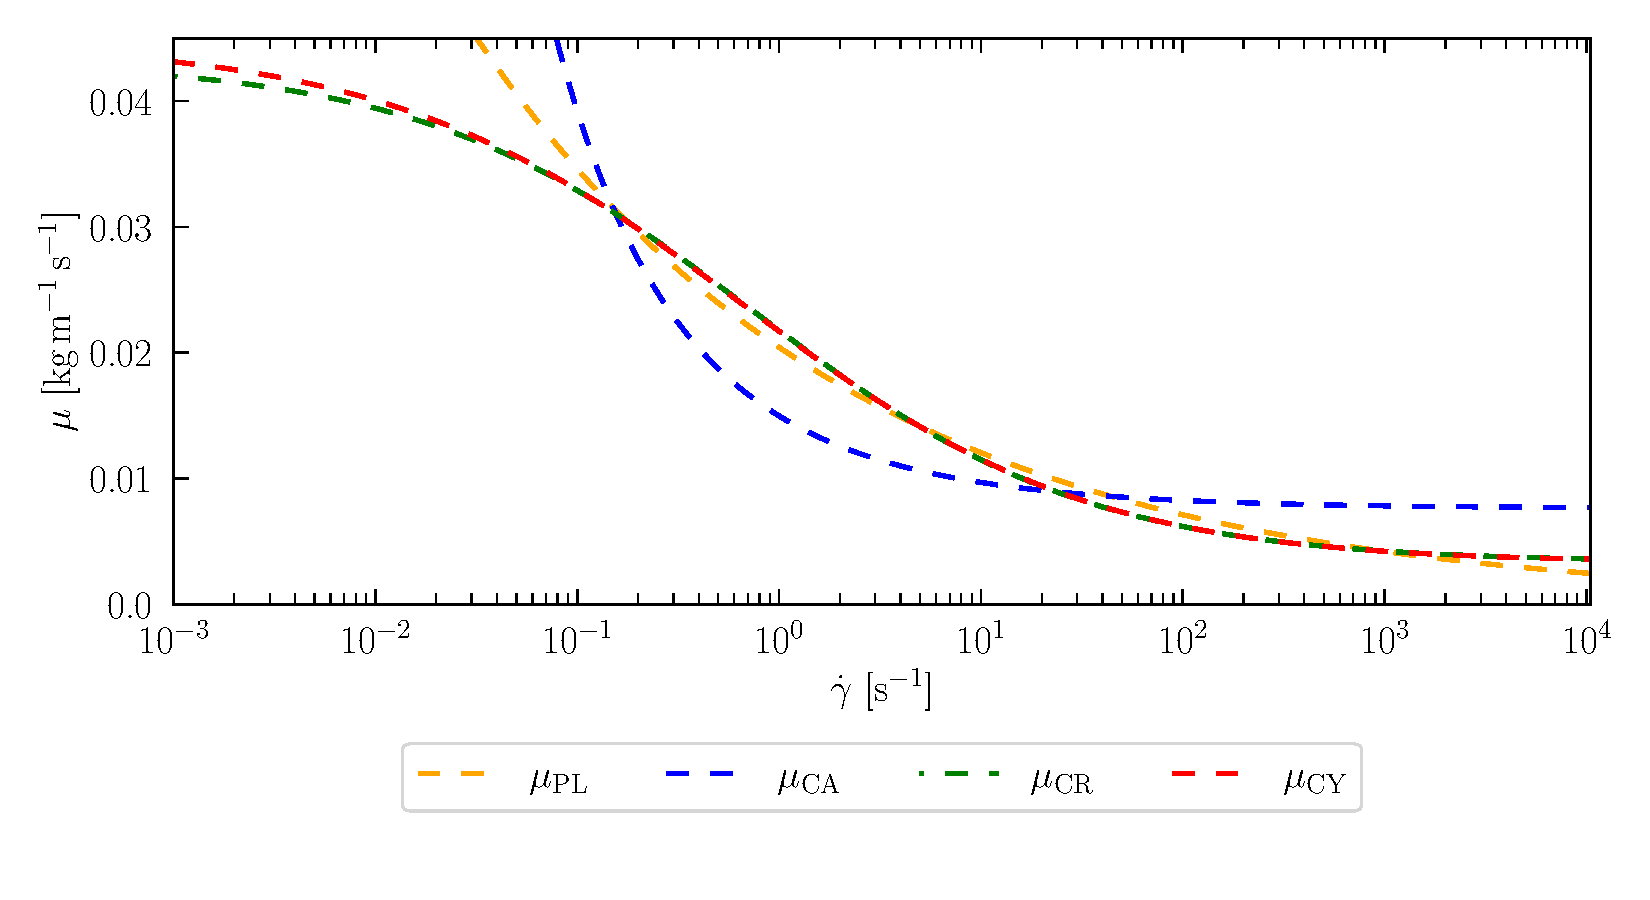
\includegraphics[width=1.0\textwidth]{Images/modely.pdf}
	\vspace{-9mm}
	\caption{Srovnání nenewtonovských modelů viskozity, konkrétní hodnoty parametrů byly převzaty z \cite{Eichler2023}. Popisy jednotlivých modelů odpovídají definujícím vztahům
    \eqref{eq:power-law}, \eqref{eq:Casson}, \eqref{eq:cross} a \eqref{eq:C-Y}}.
	\label{fig:vs}
\end{figure}

Podotkněme, že v rámci této práce budeme dále uvažovat krev výhradně jako newtonovskou tekutinu.

\section*{\fontsize{11}{15}\selectfont Turbulentní proudění}
Proudění krve je ve většině případů aproximovatelné pomocí laminárního proudění \cite{Sequeira}. V některých případech však v cévním proudění dochází k výskytu turbulencí a chaotického chování \cite{Saqr2020}. Jedna z~oblastí, kde lze turbulence pozorovat, je oblast nacházející se za cévní stenózou\footnote{Stenóza cévy je onemocnění, při němž dochází k jejímu lokálnímu zúžení  \cite{Carabello2009}.} \cite{Jain2022}. Rychlost proudění krve ve zúžené oblasti může výrazně vzrůstat, zmenšení průměru cévy však zajistí, že proudění setrvá v této části zúžení laminární \cite{Sequeira}. Avšak bezprostředně za zúžením rychlost proudění zůstavá zvýšená i~v~oblasti s původním průměrem, což může vést ke vzniku vírů a změně režimu proudění \cite{Saloner2019, Varghese2003}.

Výskyt turbulentního proudění je z fyziologického hlediska nežádoucí, jelikož je často doprovázen značnou disipací kinetické energie, kvůli níž můžou být části oběhové soustavy více namáhány. Mimoto cévní oblasti s výskytem turbulencí vykazují zvýšenou námahu na stěny cév, což může vyústit až k~narušení tkáně a k nemocem jako je např. arterioskleróza. Je tedy žádoucí turbulence v proudění krve minimalizovat \cite{Saloner2019, Kameneva2004}. 

\section{Předpoklady matematického modelu v této práci}\label{pred}
Na závěr shrneme, jaké dodatečné předpoklady budeme uvažovat v našem systému. Díky těmto předpokladům se řešení systému \eqref{NS} zjednoduší. Konkrétně budeme v rámci této práce uvažovat pouze izotermální systém (tj. jeho teplota je v čase konstantní), na který nepůsobí žádné vnější síly. Uvažovaná tekutina je dále nestlačitelná, newtonovská a s konstantní dynamickou viskozitou.

Budeme uvažovat obdélníkovou oblast $ \Omega \subset \mathbb{R}^2 $, $ \Omega = (0, L_1) \times (0, L_2) $, kde $ L_1, L_2 $ \si{[m]} jsou velikosti stran obdélníka, a časový interval $ \mathcal{I} = \langle 0, T \rangle,$ kde $ T > 0$. Označíme 

Rovnice \eqref{NS} řešené na $ \Omega \times \mathcal{I} $ se s uvažovanými předpoklady redukují na \cite{Schlichting}

\begin{subequations}\label{NS s predpoklady}
	\begin{gather}
	\label{a s predpoklady}
    \nabla \cdot \vec{u} = 0, \\[5pt]
	\label{b s predpoklady}
	\rho \frac{\text{D} \vec{u}}{\text{D} t} = - \nabla p + \mu \Delta \vec{u},
	\end{gather}
\end{subequations}
kde jsme využili zápisu pomocí operátoru materiálové derivace 
\begin{equation}
	\dfrac{\text{D}}{\text{D} t} \coloneqq \dfrac{\partial}{\partial t} + \vec{u} \cdot \nabla.
\end{equation}

Označíme $ \partial \Omega_{\text{in}} $ část hranice oblasti $ \Omega $, kde předepisujeme okrajovou podmínku na vstupu, dále $ \partial \Omega_{\text{out}} $ část hranice oblasti $ \Omega $, kde předepisujeme okrajovou podmínku na výstupu, a $ \partial \Omega_{\text{w}} $ část hranice, kde se nachází rozhraní mezi tekutinou a tělesem a kde uvažujeme no-slip okrajovou podmínku. Poté rovnice jsou rovnice \eqref{NS s predpoklady} doplněny počátečními a okrajovými podmínkami
\begin{subequations}\label{eq:okrajovky}
	\begin{alignat}{3}
	&\vec{u} = \vec{u}_{\text{ini}},  &p = p_{\text{ini}} \hspace{5mm} &\text{na } \ \Omega \times \mathcal{I}\\[3pt]
    &(\nabla p - \nu \Delta \vec{u}) \cdot \vec{n}  = 0, &\vec{u} = \vec{u}_{\text{in}} \hspace{5mm} &\text{na } \ \partial \Omega_{\text{in}} \times \mathcal{I}\\[3pt]
	&\vec{u} = \vec{0}, \, &\nabla p \cdot \vec{n} = 0 \hspace{5mm} &\text{na } \ \partial \Omega_{\text{w}} \times \mathcal{I}\\[3pt]
    &p = p_{\text{out}}, &\nabla u_i \cdot \vec{n} = 0 \hspace{5mm} &\text{na } \ \partial \Omega_{\text{out}} \times \mathcal{I}, \, i = 1, 2 \ ,
	\end{alignat}
\end{subequations}
kde $ \vec{n} $ je jednotkový vnější normálový vektor hranice uvažované oblasti, $ \vec{u}_{\text{ini}}$ \si{[m.s^{-1}]} resp. $ p_{\text{ini}} $ \si{[kg.m^{-1}.s^{-2}]} je počáteční rychlost, resp. počáteční tlak, dále $ \vec{u}_{\text{in}}$ \si{[m.s^{-1}]} je rychlost předepsaná na vstupu a $ p_{\text{out}} $~\si{[kg.m^{-1}.s^{-2}]} je tlak předepsaný na výstupu. Počáteční a okrajové podmínky jsou dále diskutovány v sekci~\ref{pocatecni a okrajove podminky}.